\begin{figure*}[t]\centering
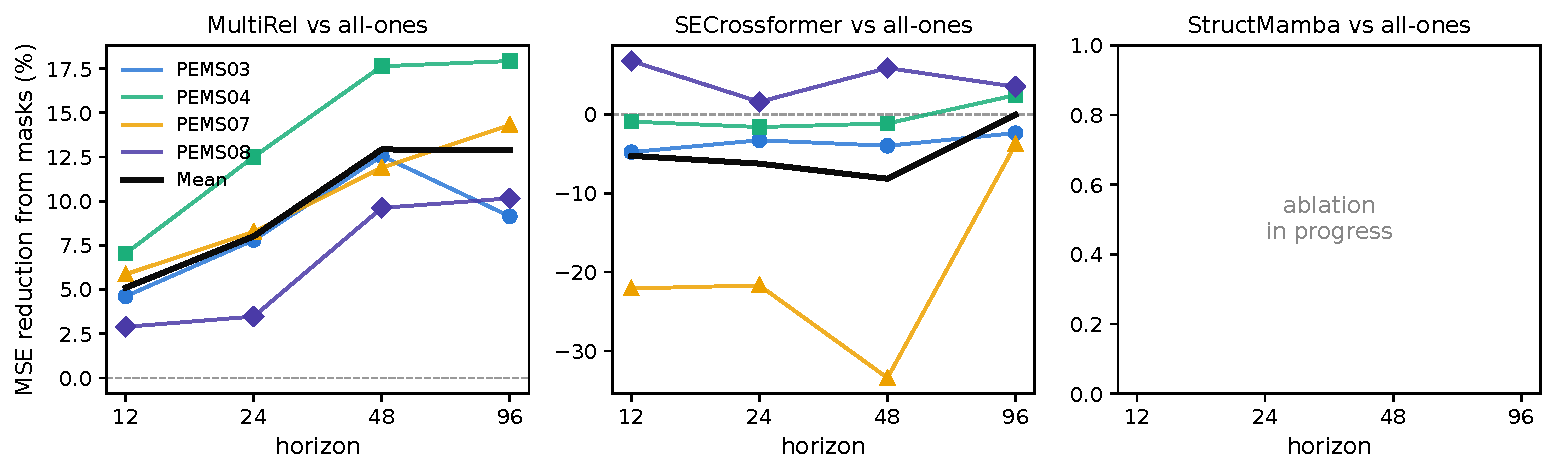
\includegraphics[width=0.98\textwidth]{figs/fig_framework_gains.pdf}
\caption{The MRMA masks in isolation: relative MSE reduction of each instantiation
over its own all-ones-mask control (same parameters and recipe, structure removed)
vs.\ forecast horizon, per PEMS dataset (thin) and averaged (thick). On the
single-stage attention backbone (\mr{}) the masks help in every cell and the margin
grows with horizon; on CrossFormer's two-stage attention the benefit is small and
mixed, localising \emph{where} the structural prior pays off.}
\label{fig:framework_gains}
\end{figure*}

\begin{table*}[t]
\centering
\caption{Mean MSE over 3 seeds, pred-12. All models re-run by us under the
shared protocol (Sec.~\ref{sec:experiments}).
Models: DLinear~\cite{zeng2023transformers}, PatchTST~\cite{nie2022time},
Autoformer~\cite{wu2021autoformer}, FEDformer~\cite{zhou2022fedformer},
Stationary~\cite{liu2022non}, TimesNet~\cite{wu2023timesnet},
CrossFormer~\cite{zhang2023crossformer}, \itrans~\cite{liu2023itransformer}.
$^\S$: CrossFormer PEMS07 has $44\%$ seed spread (seeds 0.0579--0.0836);
all other cells have seed spread below $10\%$.
Bold: best per dataset.}
\label{tab:pred12}
\footnotesize
\setlength{\tabcolsep}{3pt}
\begin{tabular}{l|cc|ccc|cc|c|c}
\toprule
 & \multicolumn{2}{c|}{Channel-indep.} & \multicolumn{3}{c|}{Transformer (decomp.)} & \multicolumn{2}{c|}{Seq./Freq.} & & \\
Dataset & DLinear & PatchTST & Autoformer & FEDformer & Stationary & TimesNet & CrossFormer & \itrans{} & \mr{} \\
\midrule
PEMS03 & 0.1048 & 0.0875 & 0.1949 & 0.1069 & 0.0848 & 0.0940 & \best{0.0636} & 0.0697 & 0.0668 \\
PEMS04 & 0.1147 & 0.1093 & 0.2223 & 0.0978 & 0.0853 & 0.0955 & \best{0.0679} & 0.0894 & 0.0817 \\
PEMS07 & 0.0998 & 0.0792 & 0.1761 & 0.0974 & 0.0831 & 0.0856 & 0.0677$^\S$ & 0.0658 & \best{0.0621} \\
PEMS08 & 0.1119 & 0.0999 & 0.2629 & 0.1599 & 0.1059 & 0.1200 & 0.1368 & 0.0800 & \best{0.0770} \\
\bottomrule
\end{tabular}
\end{table*}

\begin{figure*}[t]
\centering
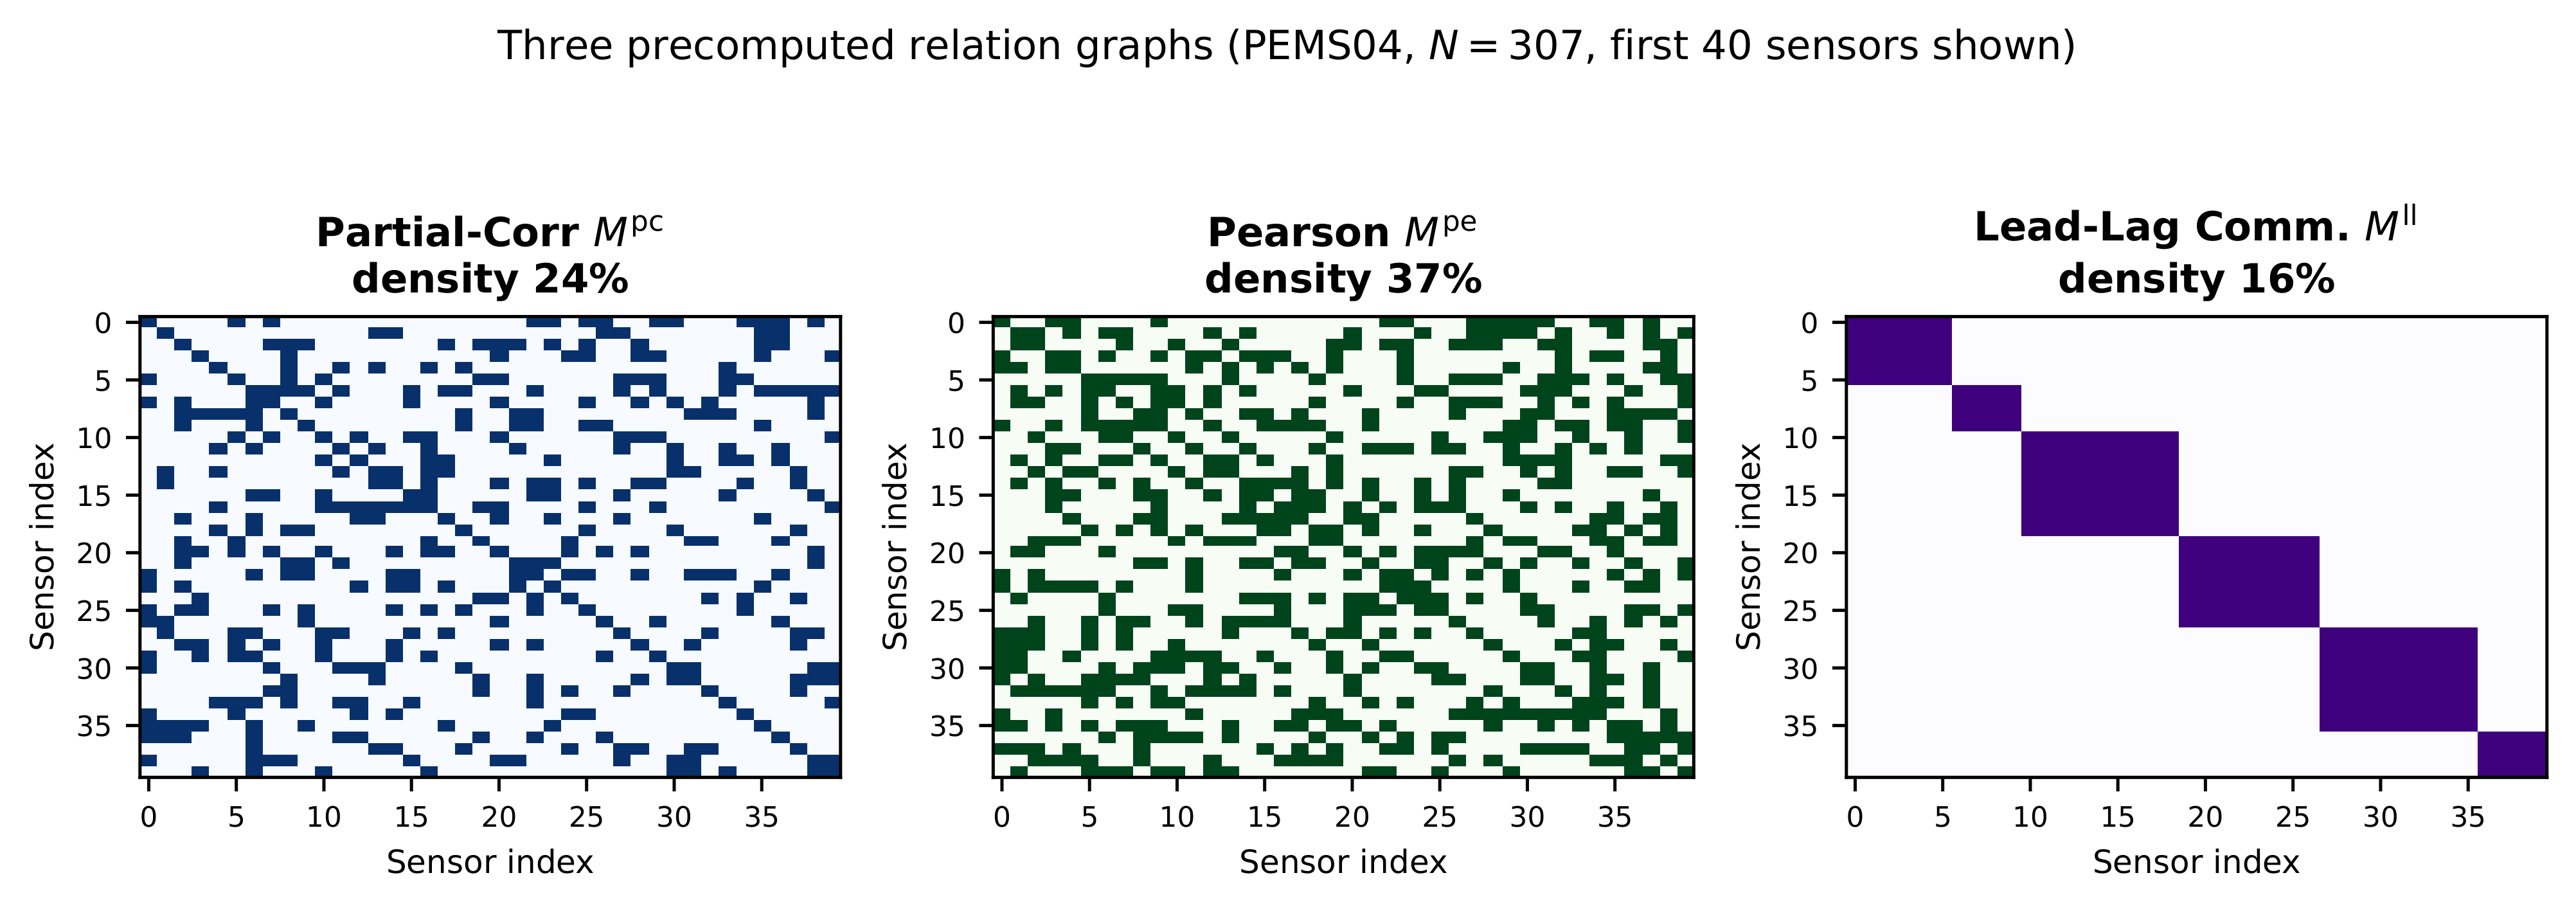
\includegraphics[width=0.85\textwidth]{fig_graphs.png}
\caption{Three precomputed relation graphs for PEMS04 ($N{=}307$, first 40 sensors shown).
\textbf{Left:} partial-correlation $M^{\text{pc}}$ (sparse, conditional links).
\textbf{Centre:} Pearson $M^{\text{pe}}$ (denser, marginal co-movement).
\textbf{Right:} lead-lag community $M^{\text{ll}}$ (block-diagonal clusters).
The three graphs encode complementary structure; their union covers a strictly
richer dependency set than any single graph alone.}
\label{fig:graphs}
\end{figure*}

\begin{table}[t]
\centering
\caption{PEMS dataset characteristics.}
\label{tab:datasets}
\small
\begin{tabular}{lrrrr}
\toprule
Dataset & $N$ & Time steps & Train & Test \\
\midrule
PEMS03 & 358 & 26{,}208 & 15{,}724 & 5{,}241 \\
PEMS04 & 307 & 16{,}992 & 10{,}195 & 3{,}398 \\
PEMS07 & 883 & 28{,}224 & 16{,}934 & 5{,}644 \\
PEMS08 & 170 & 17{,}856 & 10{,}713 & 3{,}571 \\
\bottomrule
\end{tabular}
\end{table}

\begin{figure}[t]
\centering
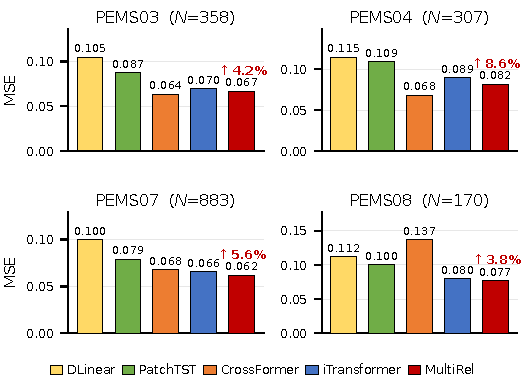
\includegraphics[width=\columnwidth]{fig_pred12.pdf}
\caption{Pred-12 MSE on the four PEMS benchmarks (selected baselines; lower is
better). \mr{} (red) achieves the lowest MSE on PEMS07/08 and beats \itrans{} everywhere; the red
$\uparrow$ label gives its relative improvement over \itrans{} (blue), as in
Table~\ref{tab:grid}.}
\label{fig:pred12}
\end{figure}

\begin{table*}[t]
\centering
\caption{Mean MSE over 3 independent seeds, varying prediction horizon.
Parentheses: \textcolor{gaincolor}{$\uparrow$X\%} = relative MSE improvement over \itrans{} (lower MSE is better).
All values self-reproduced under the shared protocol.
$^\S$: CrossFormer exhibits extreme seed instability beyond pred-12 (spreads up
to $60\%$, e.g.\ seeds $0.129$--$0.207$ at PEMS04 pred-48; \mr{} stays below
$3\%$) --- its low means at PEMS03/04 pred-96 come with this caveat.
Bold: best mean per dataset--horizon.}
\label{tab:grid}
\small
\setlength{\tabcolsep}{3.5pt}
\begin{tabular}{llcccc}
\toprule
Dataset & Model & pred-12 & pred-24 & pred-48 & pred-96 \\
\midrule
\multirow{4}{*}{PEMS03}
  & DLinear                  & 0.1048  & 0.1829  & 0.3184  & 0.4506 \\
  & CrossFormer$^\S$         & \best{0.0636}   & 0.1080  & 0.2154  & \best{0.2094}  \\
  & \itrans{}                & 0.0697  & 0.1009  & 0.1675  & 0.2693 \\
  & \mr{}                    & 0.0668\,{\scriptsize\gain{($\uparrow$4.2\%)}}
                             & \best{0.0935}\,{\scriptsize\gain{($\uparrow$7.3\%)}}
                             & \best{0.1484}\,{\scriptsize\gain{($\uparrow$11.4\%)}}
                             & 0.2458\,{\scriptsize\gain{($\uparrow$8.7\%)}} \\
\midrule
\multirow{4}{*}{PEMS04}
  & DLinear                  & 0.1147  & 0.1890  & 0.3222  & 0.4284 \\
  & CrossFormer$^\S$         & \best{0.0679}   & \best{0.0783}  & 0.1609  & \best{0.1310} \\
  & \itrans{}                & 0.0894  & 0.1262  & 0.2019  & 0.3166 \\
  & \mr{}                    & 0.0817\,{\scriptsize\gain{($\uparrow$8.6\%)}}
                             & 0.1075\,{\scriptsize\gain{($\uparrow$14.8\%)}}
                             & \best{0.1605}\,{\scriptsize\gain{($\uparrow$20.5\%)}}
                             & 0.2485\,{\scriptsize\gain{($\uparrow$21.5\%)}} \\
\midrule
\multirow{4}{*}{PEMS07}
  & DLinear                  & 0.0998  & 0.1891  & 0.3772  & 0.5778 \\
  & CrossFormer$^\S$         & 0.0677  & 0.1358  & 0.2041  & 0.2547 \\
  & \itrans{}                & 0.0658  & 0.0948  & 0.1500  & 0.2296 \\
  & \mr{}                    & \best{0.0621}\,{\scriptsize\gain{($\uparrow$5.6\%)}}
                             & \best{0.0871}\,{\scriptsize\gain{($\uparrow$8.1\%)}}
                             & \best{0.1320}\,{\scriptsize\gain{($\uparrow$12.0\%)}}
                             & \best{0.1953}\,{\scriptsize\gain{($\uparrow$14.9\%)}} \\
\midrule
\multirow{4}{*}{PEMS08}
  & DLinear                  & 0.1119  & 0.1965  & 0.3860  & 0.6456 \\
  & CrossFormer$^\S$         & 0.1368  & 0.1637  & 0.1904  & \best{0.2156} \\
  & \itrans{}                & 0.0800  & 0.1177  & 0.2063  & 0.3833 \\
  & \mr{}                    & \best{0.0770}\,{\scriptsize\gain{($\uparrow$3.8\%)}}
                             & \best{0.1109}\,{\scriptsize\gain{($\uparrow$5.8\%)}}
                             & \best{0.1801}\,{\scriptsize\gain{($\uparrow$12.7\%)}}
                             & 0.3285\,{\scriptsize\gain{($\uparrow$14.3\%)}} \\
\bottomrule
\end{tabular}
\end{table*}

\begin{figure}[t]
\centering
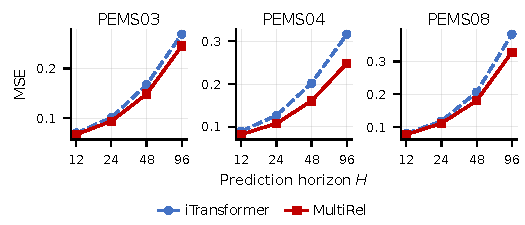
\includegraphics[width=\columnwidth]{fig_horizon.pdf}
\caption{MSE vs.\ prediction horizon (lower is better) for \mr{} (solid red)
and \itrans{} (dashed blue) on PEMS03, PEMS04, and PEMS08. The gap widens as the
horizon grows, confirming that spatial structure becomes increasingly informative
as short-range temporal autocorrelation fades.}
\label{fig:horizon}
\end{figure}

\begin{table*}[t]
\centering
\caption{Relation ablation, pred-12, 3 seeds ($d{=}512$ configuration).
Single-relation models activate one mask type only; the other two heads use full
(unmasked) attention. \itrans{} re-run under the same config.}
\label{tab:ablation}
\small
\begin{tabular}{lccccc}
\toprule
Dataset & \itrans & \mr-PC & \mr-PE & \mr-LL & \mr{} (3-rel) \\
\midrule
PEMS04 & 0.0881 & 0.0850\,{\scriptsize\gain{$\uparrow$3.5\%}} & 0.0817\,{\scriptsize\gain{$\uparrow$7.3\%}} & 0.0863\,{\scriptsize\gain{$\uparrow$2.0\%}} & \best{0.0794}\,{\scriptsize\gain{$\uparrow$9.9\%}} \\
PEMS08 & 0.0799 & 0.0792\,{\scriptsize\gain{$\uparrow$0.9\%}} & 0.0776\,{\scriptsize\gain{$\uparrow$2.9\%}} & 0.0791\,{\scriptsize\gain{$\uparrow$1.0\%}} & \best{0.0774}\,{\scriptsize\gain{$\uparrow$3.1\%}} \\
\bottomrule
\end{tabular}
\end{table*}

\begin{figure}[t]
\centering
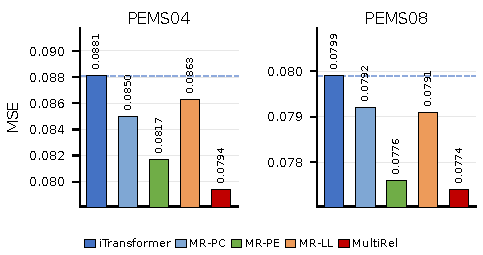
\includegraphics[width=0.92\columnwidth]{fig_ablation.pdf}
\caption{Relation ablation on PEMS04 (left) and PEMS08 (right) at the $d{=}512$
ablation configuration, matching Table~\ref{tab:ablation}; lower is better.
Every single-relation variant improves on \itrans{} (dashed reference line), and
the full 3-relation \mr{} (rightmost bar) achieves the lowest MSE in both cases
at this width (see text for the $d{=}256$ caveat).}
\label{fig:ablation}
\end{figure}

\begin{table}[t]
\centering
\caption{$k$-sensitivity: \mr{} MSE on PEMS04 pred-12 (3 seeds, $d{=}512$). Bold: best.}
\label{tab:ksens}
\small
\begin{tabular}{lcccccc}
\toprule
$k$ & 5 & 10 & 15 & 20 & 25 & 30 \\
\midrule
MSE & 0.0780 & \best{0.0776} & 0.0777 & 0.0794 & 0.0785 & 0.0785 \\
\bottomrule
\end{tabular}
\end{table}

\begin{table}[t]
\centering
\caption{Graph statistics across PEMS datasets ($k{=}20$).
Density $= |E|/(N(N{-}1))$; self-loops excluded.
``Comm.'' = number of SE-agglomerative communities in $\mathbf{M}^{\text{ll}}$.
``Union\%'' = fraction of all directed pairs covered by $\mathbf{M}^{\text{pc}}\cup\mathbf{M}^{\text{pe}}\cup\mathbf{M}^{\text{ll}}$.}
\label{tab:graphstats}
\small
\setlength{\tabcolsep}{3.5pt}
\begin{tabular}{lrrrrrr}
\toprule
 & \multicolumn{2}{c}{$\mathbf{M}^{\text{pc}/\text{pe}}$} & \multicolumn{2}{c}{$\mathbf{M}^{\text{ll}}$} & \\
\cmidrule(lr){2-3}\cmidrule(lr){4-5}
Dataset & Deg. & Dens. & Deg. & Dens. & Comm. & Union\% \\
\midrule
PEMS03 (358) & 21.0 & 5.9\% & 60.9 & 17.1\% & 6  & 22.7\% \\
PEMS04 (307) & 21.0 & 6.9\% & 79.9 & 26.1\% & 4  & 32.8\% \\
PEMS07 (883) & 21.0 & 2.4\% & 133.2 & 15.1\% & 8  & 17.0\% \\
PEMS08 (170) & 21.0 & 12.4\% & 63.3 & 37.4\% & 3  & 46.5\% \\
\bottomrule
\end{tabular}
\end{table}

\begin{table}[t]
\centering
\caption{Computational cost comparison, PEMS07 pred-12 ($N{=}883$, RTX~A4000).}
\label{tab:cost}
\small
\begin{tabular}{lcrr}
\toprule
Model & Params & Time/epoch & Peak GPU \\
\midrule
DLinear        & 21.3K  & $\sim$5\,s  & 0.4\,GB \\
\itrans{}      & 1$\times$  & 45\,s      & 4.7\,GB \\
\mr{} (ours)   & 1$\times$ (identical)  & 46\,s      & 4.9\,GB \\
\bottomrule
\end{tabular}
\end{table}

\begin{table}[t]
\centering
\caption{Shared hyperparameters for \mr{} and \itrans{}.}
\label{tab:hyperparams}
\small
\begin{tabular}{ll}
\toprule
Hyperparameter & Value \\
\midrule
Encoder layers ($L$) & 3 \\
Model dimension ($d$) & 256 \\
FFN dimension ($d_{\text{ff}}$) & 512 \\
Attention heads ($h$) & 8 \\
Dropout & 0.1 \\
Normalisation & RevIN \\
Optimiser & Adam \\
Learning rate & $5{\times}10^{-4}$ \\
Epochs & 10 \\
Batch size & 8--16 (by memory footprint) \\
Input length & 96 \\
Early stopping patience & 3 \\
\midrule
$k$ (neighbourhood size) & 20 \\
Max lag $L_{\max}$ & 12 \\
\bottomrule
\end{tabular}
\end{table}

\begin{table}[t]
\centering
\caption{Cross-domain MSE at pred-96 (mean over 3 seeds).
Bold: best.
Gain column: relative MSE improvement of \mr{} over \itrans{} ($+$ = better).}
\label{tab:xdomain}
\small
\setlength{\tabcolsep}{4pt}
\begin{tabular}{lcccc}
\toprule
Dataset ($N$) & \itrans{} & \mr{} & Gain & $k$ \\
\midrule
Solar ($N{=}137$)    & \best{0.2176} & 0.2230 & $-$2.5\% & 20 \\
ETTh1 ($N{=}7$)      & 0.3977 & \best{0.3972} & $\approx$0\% & 3  \\
ETTm1 ($N{=}7$)      & 0.3437 & \best{0.3422} & $+$0.4\% & 3  \\
\bottomrule
\end{tabular}
\end{table}
